



\begin{frame}{Simulations}
\begin{itemize}
\item VMS linearized coupled sd7003s - Re $\num{60000}$ - AoA $\ang{4}$ 
\item VMS linearized segregated DU89 - Re $\num{250000}-\num{500000}$ - AoA $\ang{1}-\ang{5}$ 
\end{itemize}
\end{frame}

\begin{frame}{Models}
sd7003s - Re $\num{60000}$ - AoA $\ang{4}$ 
\begin{figure}[h]
     \centering          
         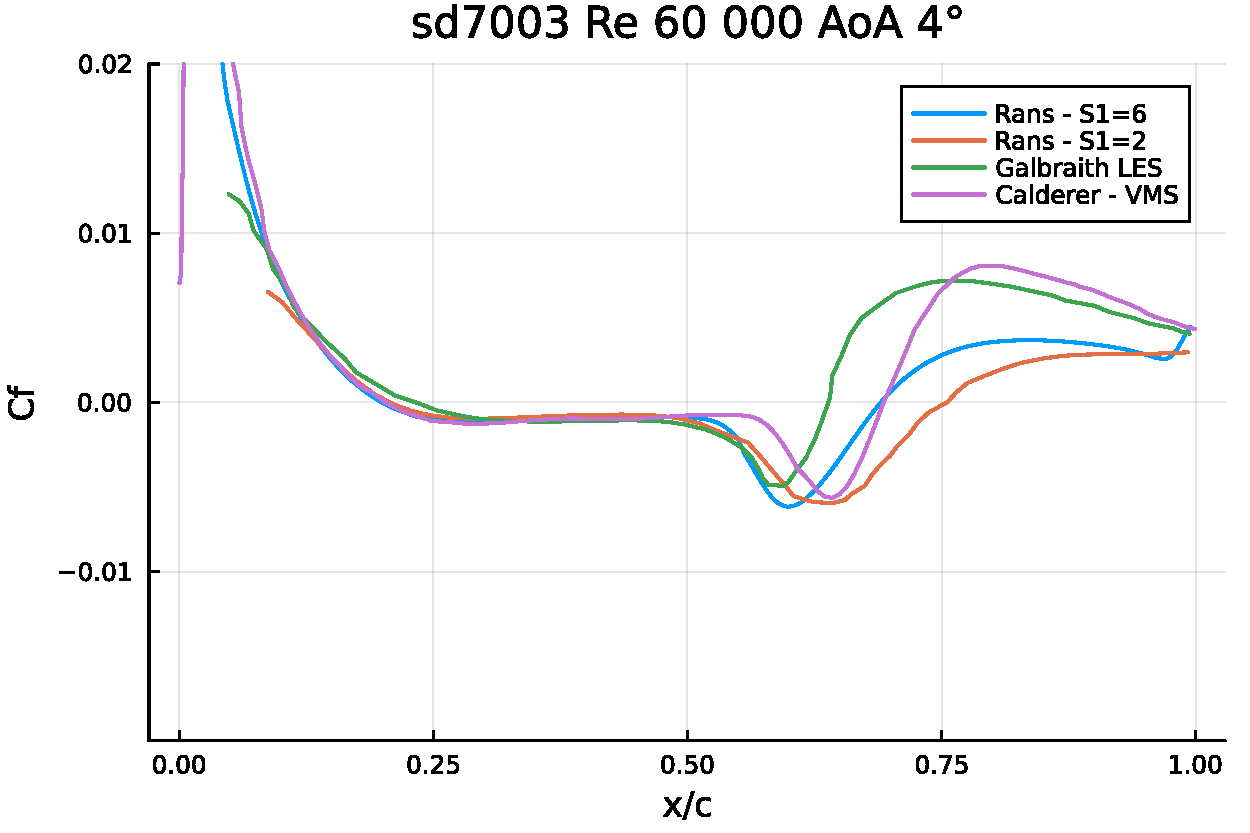
\includegraphics[width=0.65\textwidth]{ sd7003_differentmodels.pdf}
         \caption{Different model provides different results. RANs use $\gamma -Re_ \theta$ model.}
     \end{figure} 
\end{frame}

\begin{frame}{VMS linearized coupled sd7003s}
Copuled: velocity and pressure are solved at the same time.
Re $\num{60000}$ - AoA $\ang{4}$ . Initialization with velocity-ramping
\begin{figure}[h]
     \centering          
     \begin{subfigure}[h]{0.45\textwidth}
              \centering
         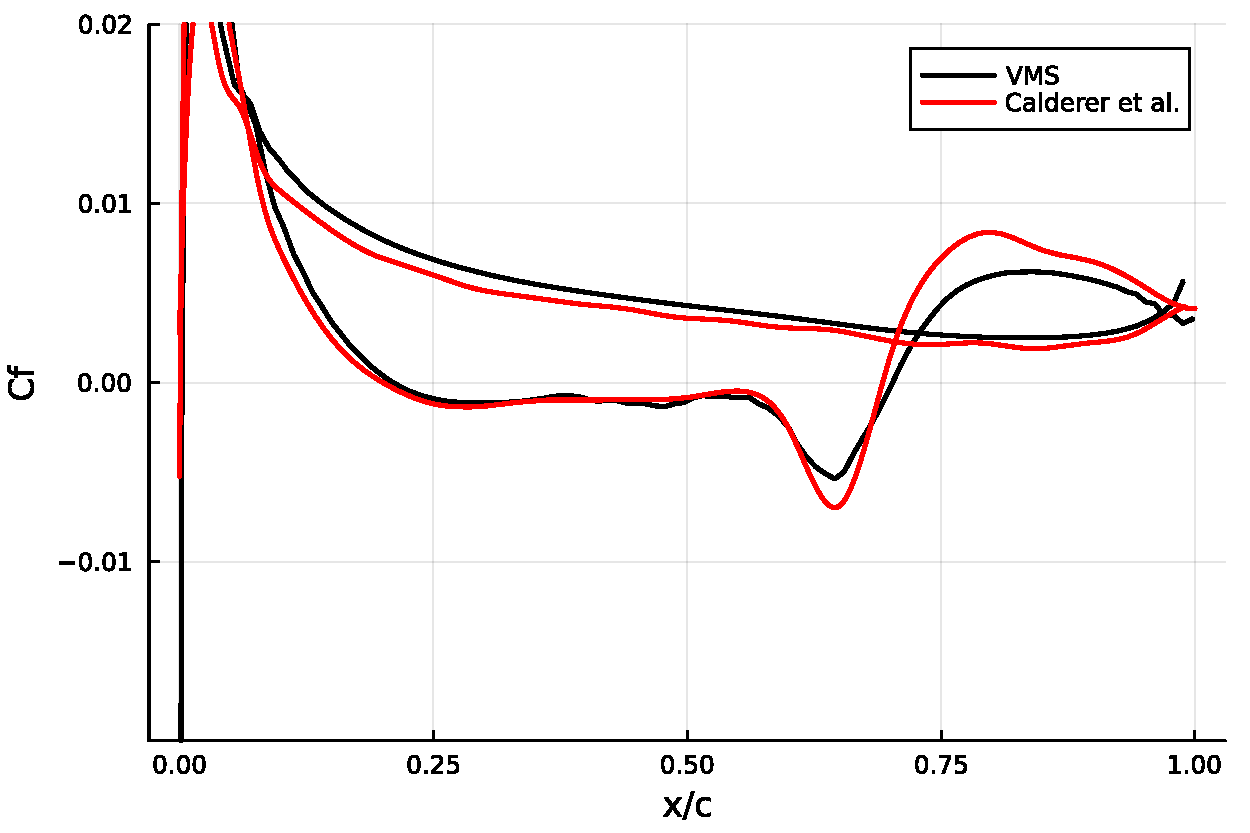
\includegraphics[width=\textwidth]{sd7003_cf.pdf}
    \end{subfigure}
          \hfill
     \begin{subfigure}[h]{0.45\textwidth}
      \centering
         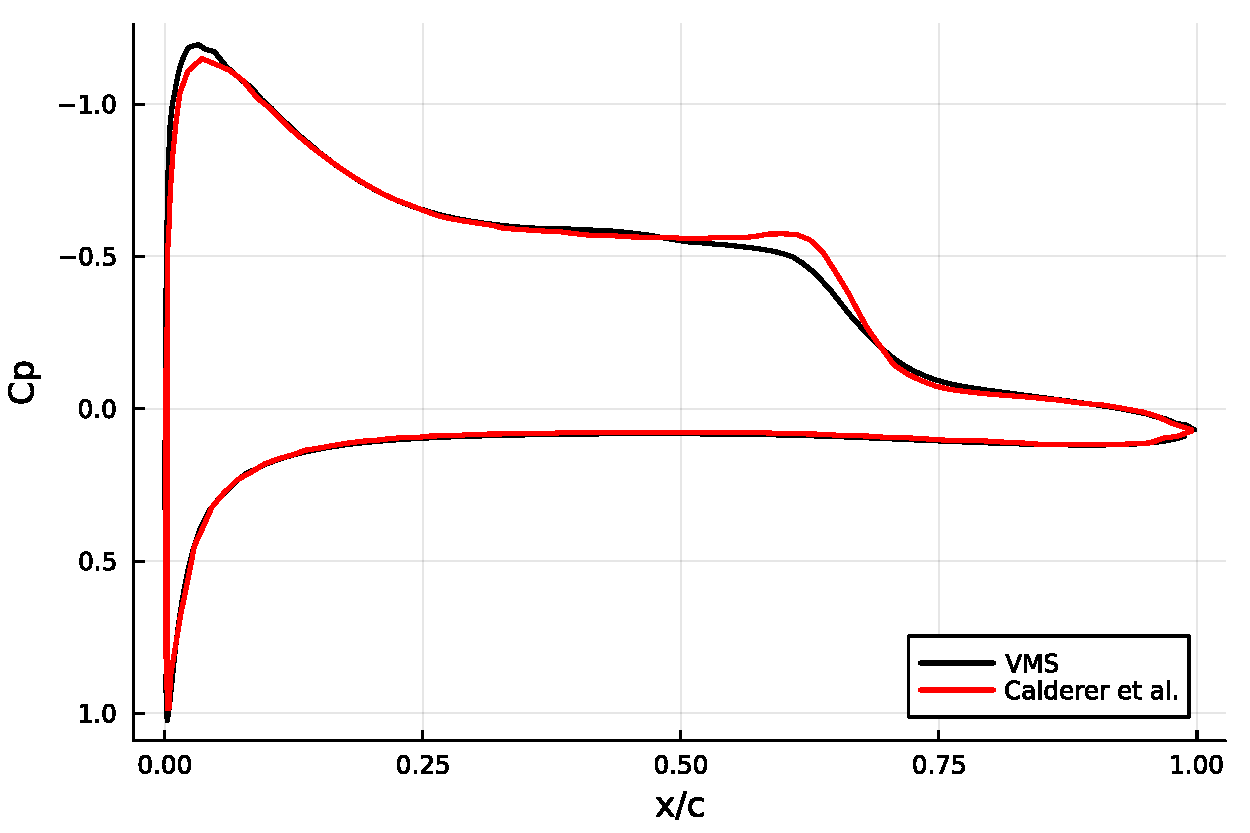
\includegraphics[width=\textwidth]{sd7003_cp.pdf}
     \end{subfigure}
\caption{Comparison with VMS literature results}
     \end{figure} 
     
\end{frame}

\begin{frame}{ VMS linearized coupled sd7003s}
\begin{figure}[h]
     \centering          
         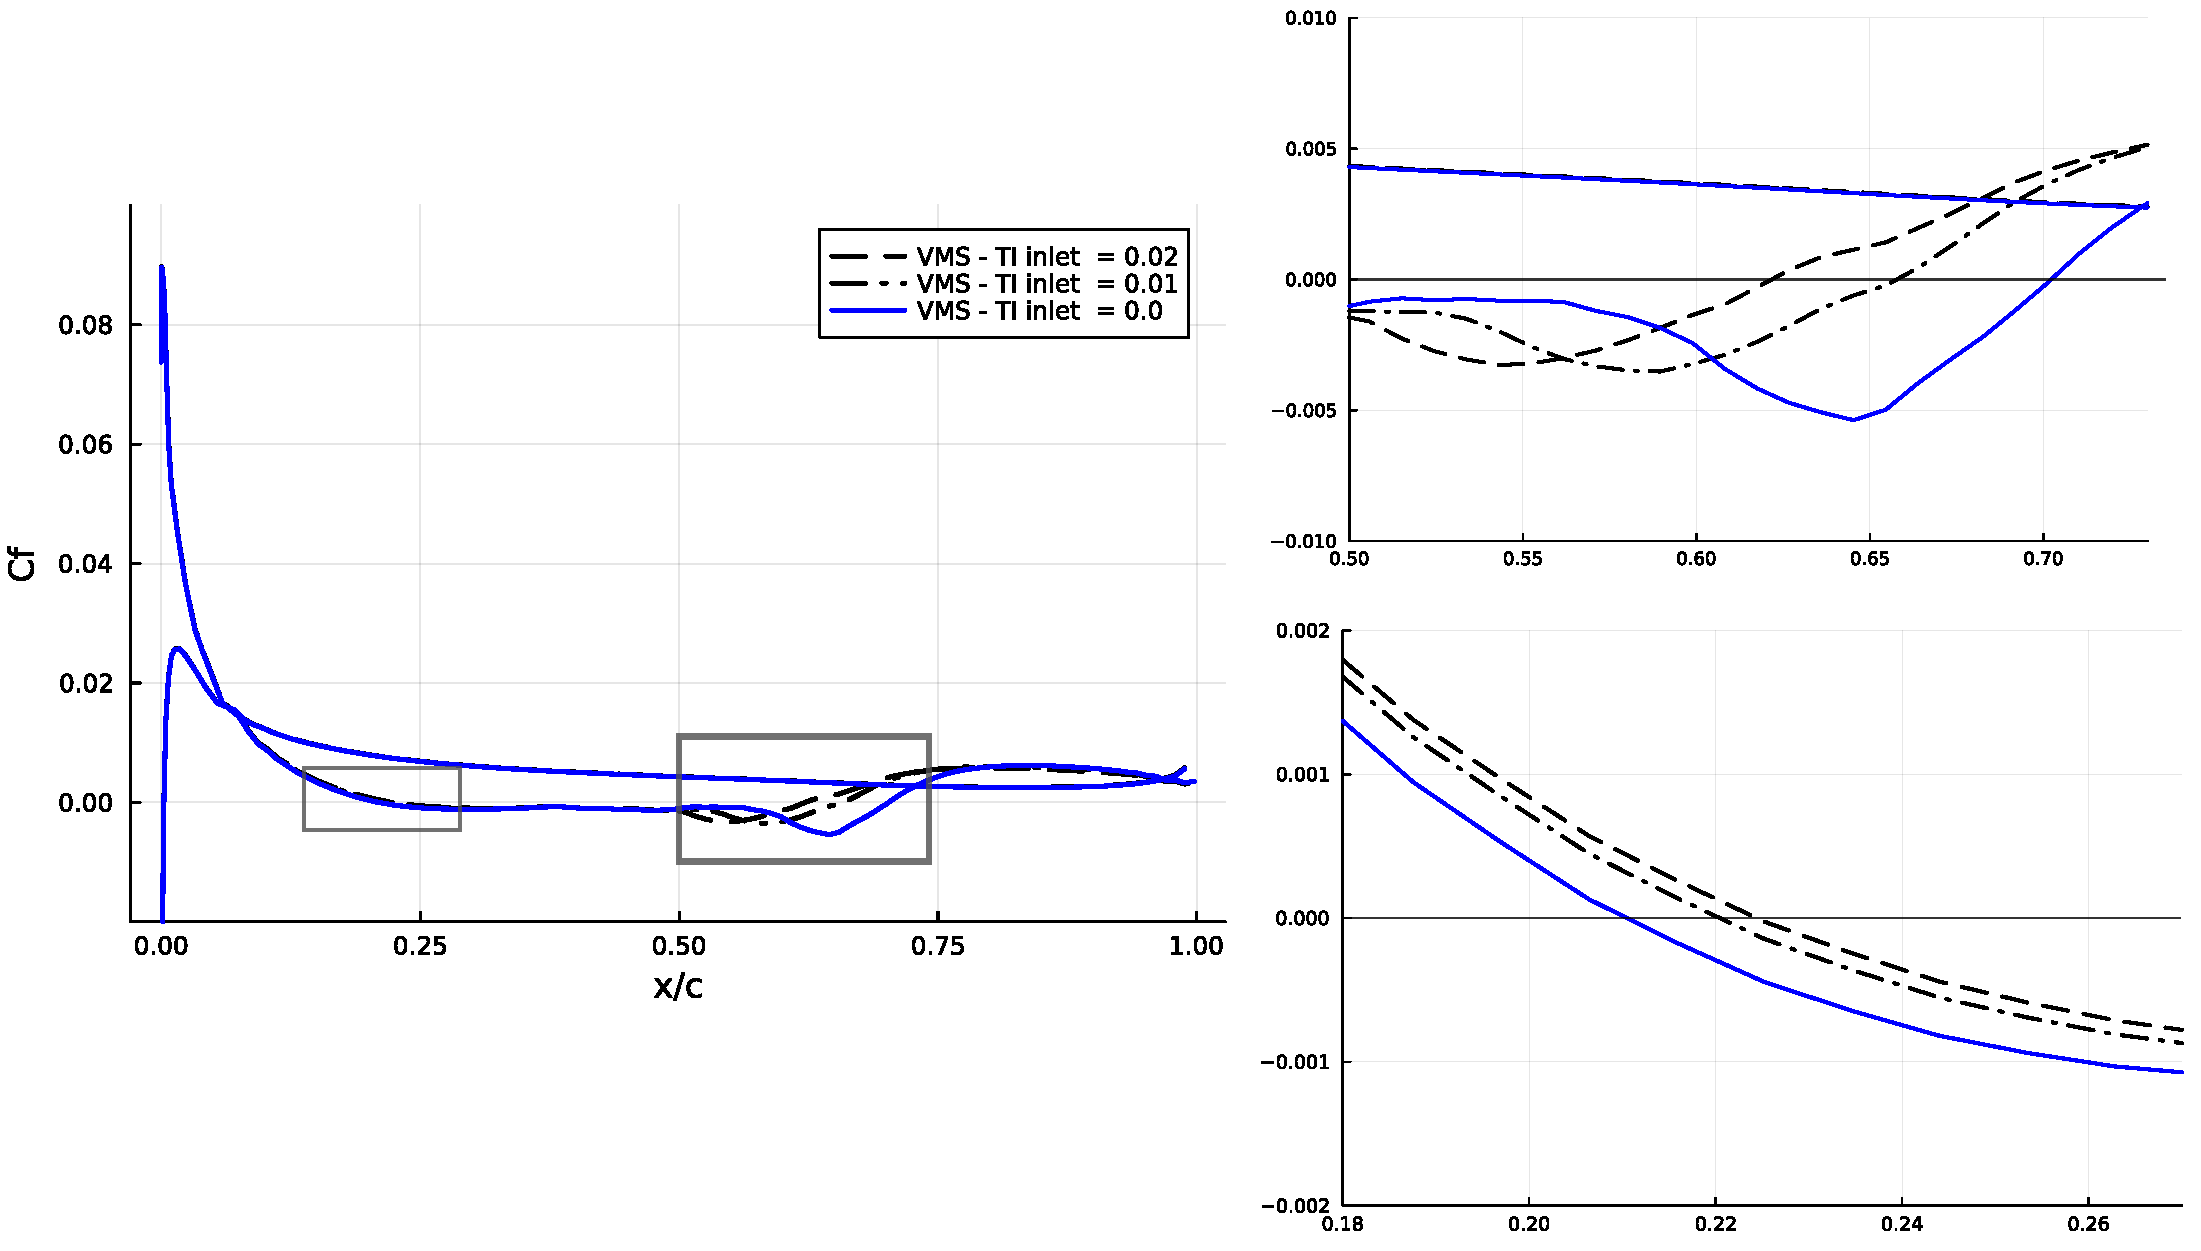
\includegraphics[width=0.8\textwidth]{SD7003_Cf_zoom.pdf}
         \caption{Bubble position function of freestream turbulence intensity}
     \end{figure} 
\end{frame}




\begin{frame}{VMS Linearized-Segregated}
Segregated: each time step pressure and velocity system are solved one after the other multiple times. It is possible to re-use the matrices and preconditioner. It is an iterative method.

\end{frame}




\begin{frame}{VMS Linearized-Segregated}
PhD research aims to simulate new a new airfoil.
Re $\num{250000}$ - AoA $\ang{1}$ 

\begin{figure}[h]
     \centering          
     \begin{subfigure}[h]{0.45\textwidth}
              \centering
         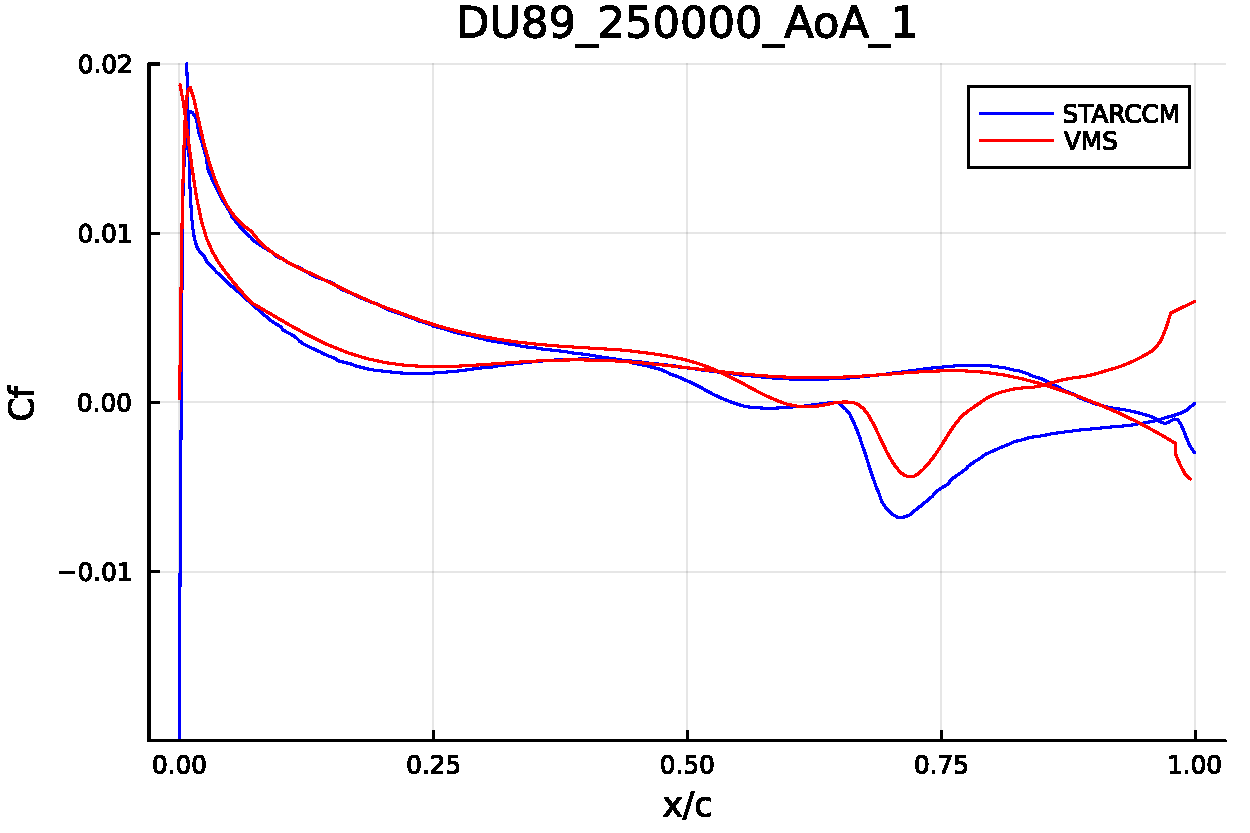
\includegraphics[width=\textwidth]{DU89_250000_AoA_1_Cf.pdf}
    \end{subfigure}
          \hfill
     \begin{subfigure}[h]{0.45\textwidth}
      \centering
         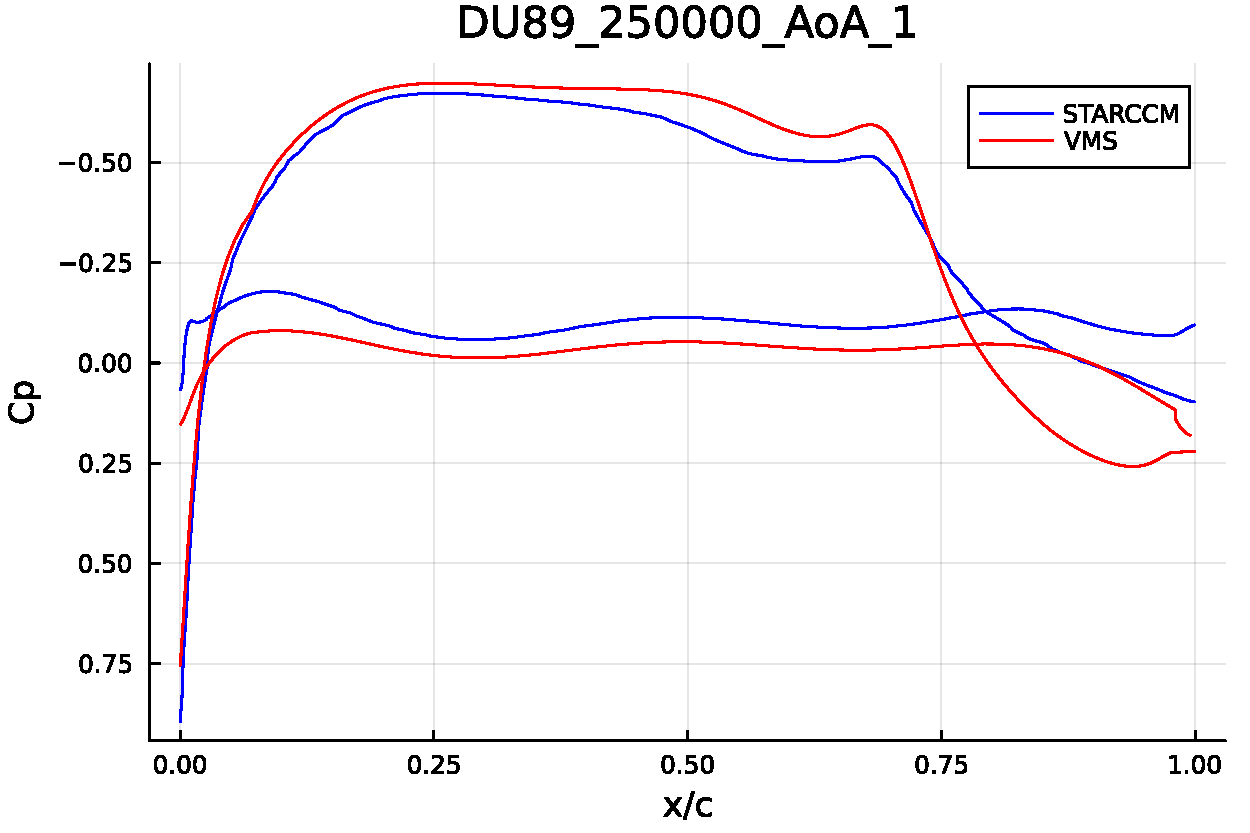
\includegraphics[width=\textwidth]{DU89_250000_AoA_1_Cp.pdf}
     \end{subfigure}
     \end{figure} 
 \end{frame}

\begin{frame}{VMS Linearized-Segregated}
Re $\num{250000}$ - AoA $\ang{5}$ 
\begin{figure}[h]
     \centering          
     \begin{subfigure}[h]{0.45\textwidth}
              \centering
         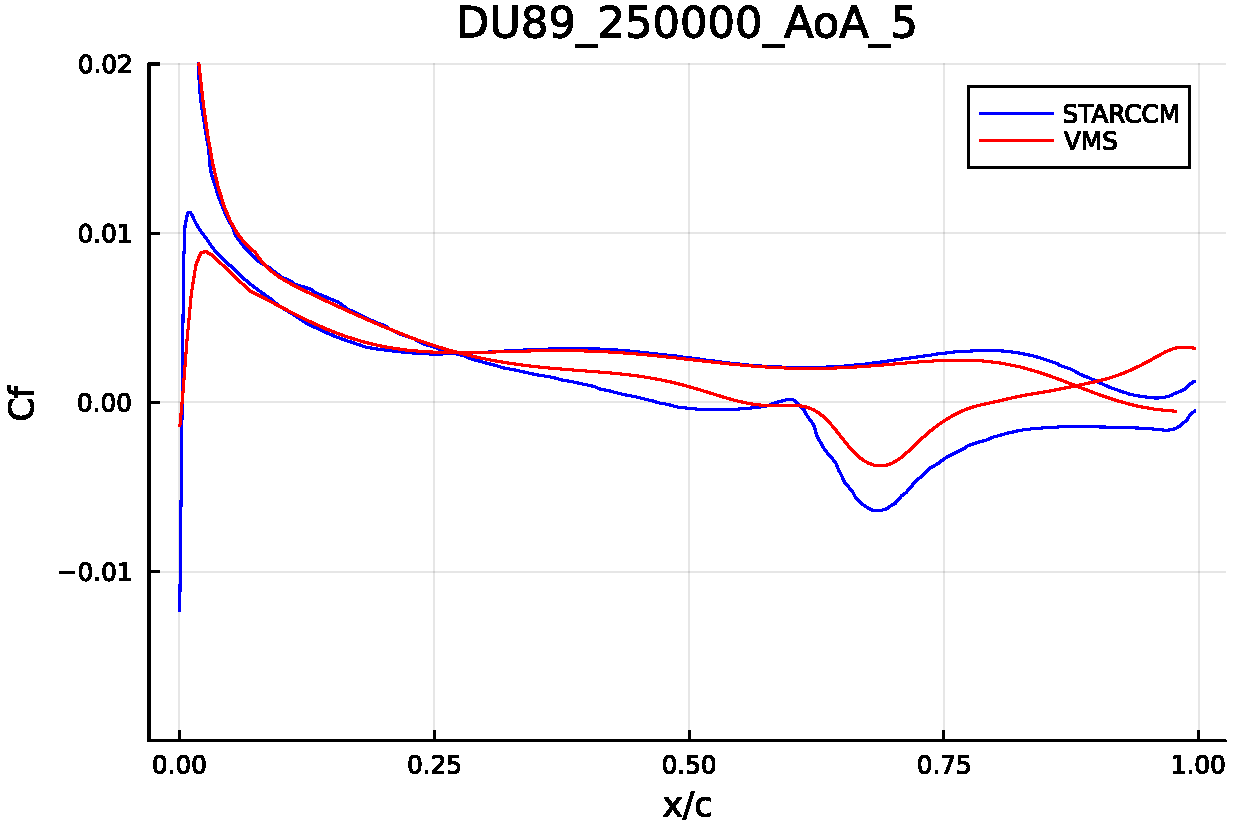
\includegraphics[width=\textwidth]{DU89_250000_AoA_5_Cf.pdf}
    \end{subfigure}
          \hfill
     \begin{subfigure}[h]{0.45\textwidth}
      \centering
         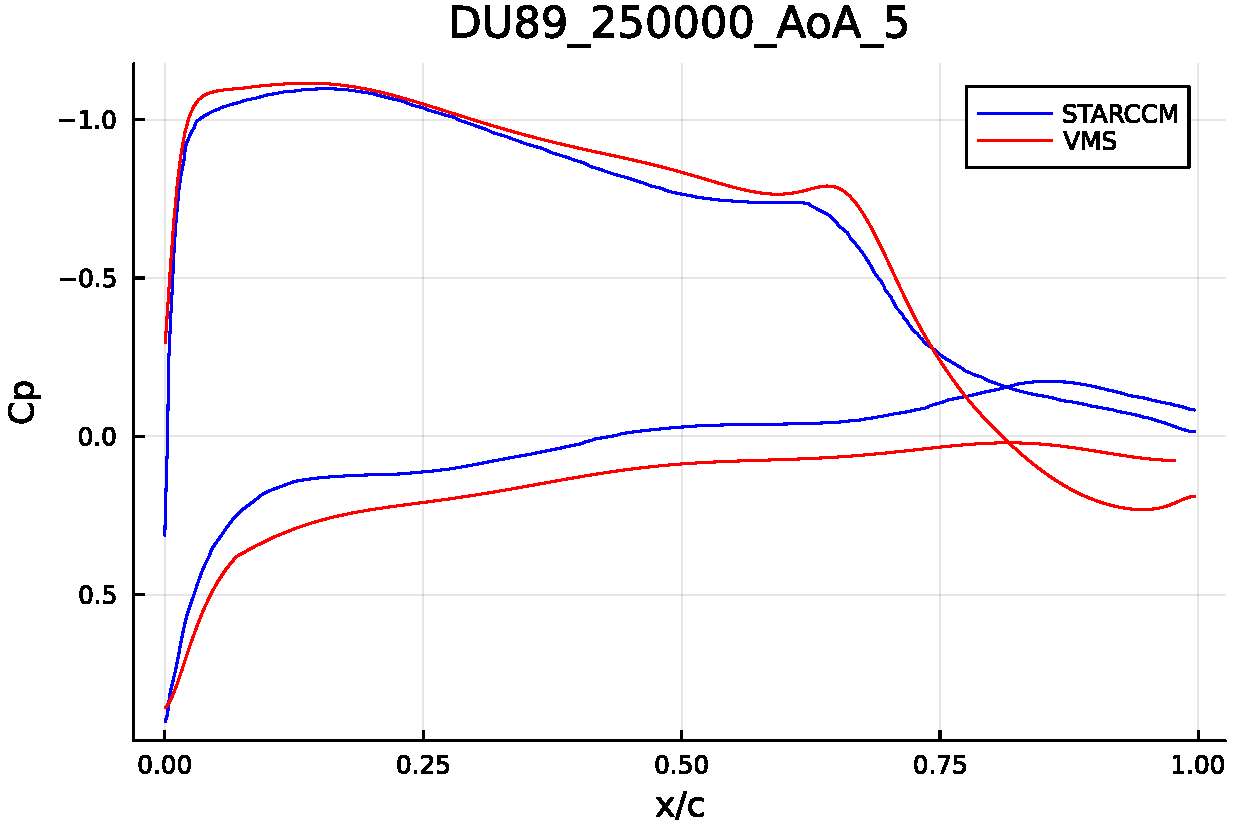
\includegraphics[width=\textwidth]{DU89_250000_AoA_5_Cp.pdf}
     \end{subfigure}
     \end{figure} 
 \end{frame}

\begin{frame}{VMS Linearized-Segregated}
Re $\num{500000}$ - AoA $\ang{1}$ 
\begin{figure}[h]
     \centering          
     \begin{subfigure}[h]{0.45\textwidth}
              \centering
         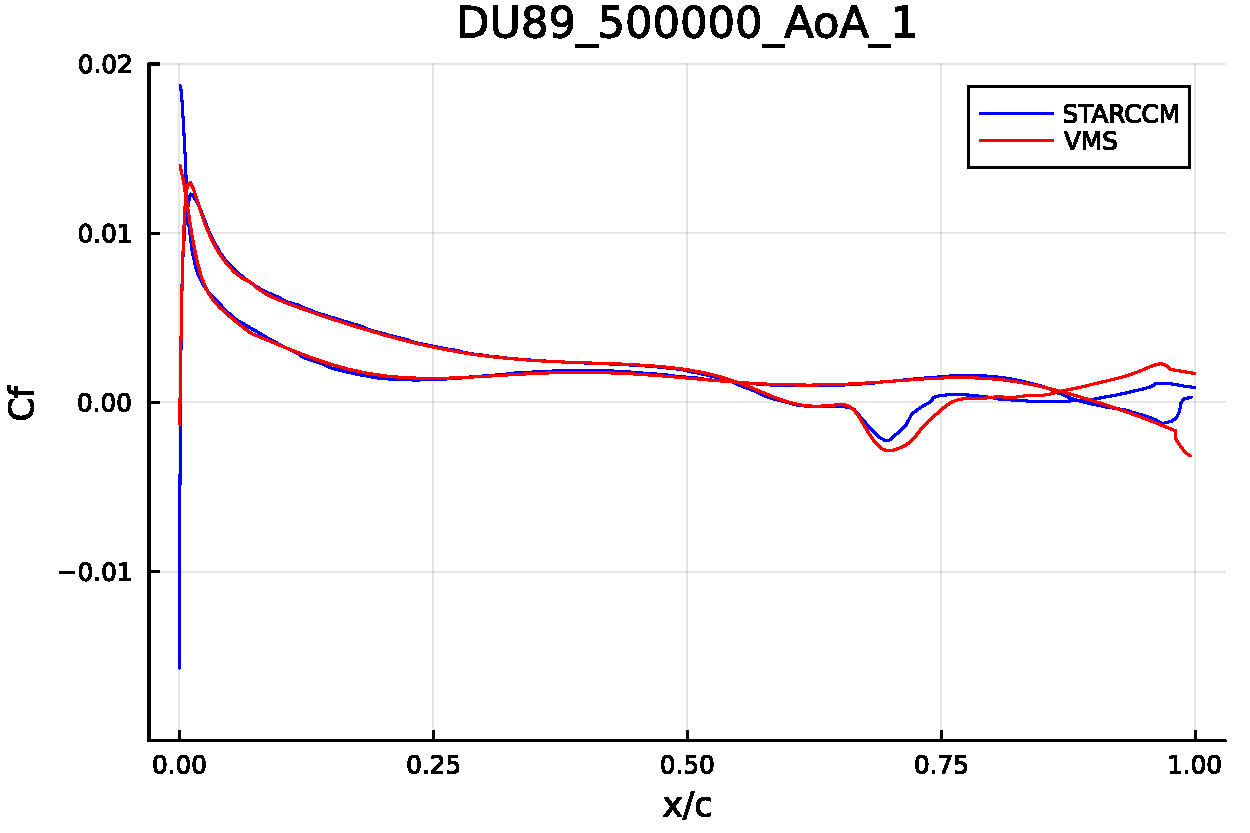
\includegraphics[width=\textwidth]{DU89_500000_AoA_1_Cf.pdf}
    \end{subfigure}
          \hfill
     \begin{subfigure}[h]{0.45\textwidth}
      \centering
         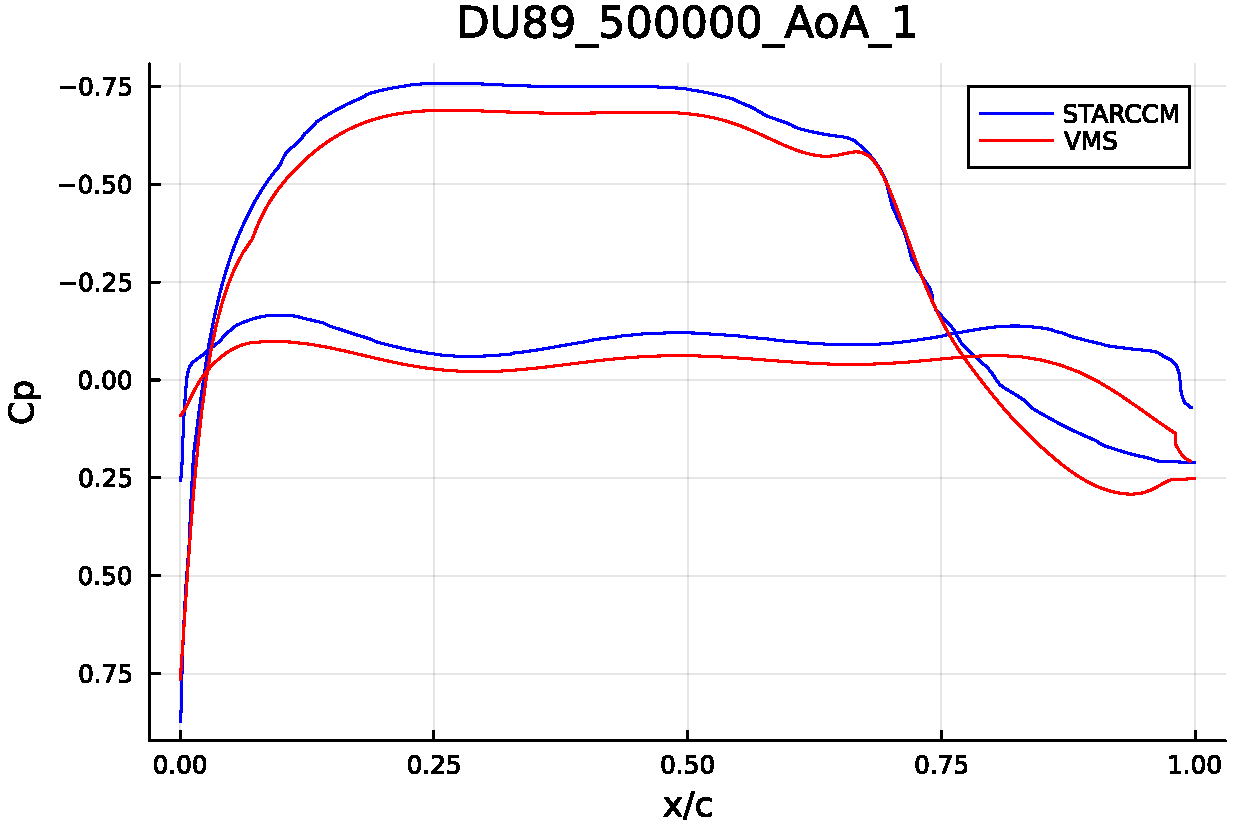
\includegraphics[width=\textwidth]{DU89_500000_AoA_1_Cp.pdf}
     \end{subfigure}
     \end{figure} 
 \end{frame}

\begin{frame}{VMS Linearized-Segregated}
Re $\num{500000}$ - AoA $\ang{5}$ 
\begin{figure}[h]
     \centering          
     \begin{subfigure}[h]{0.45\textwidth}
              \centering
         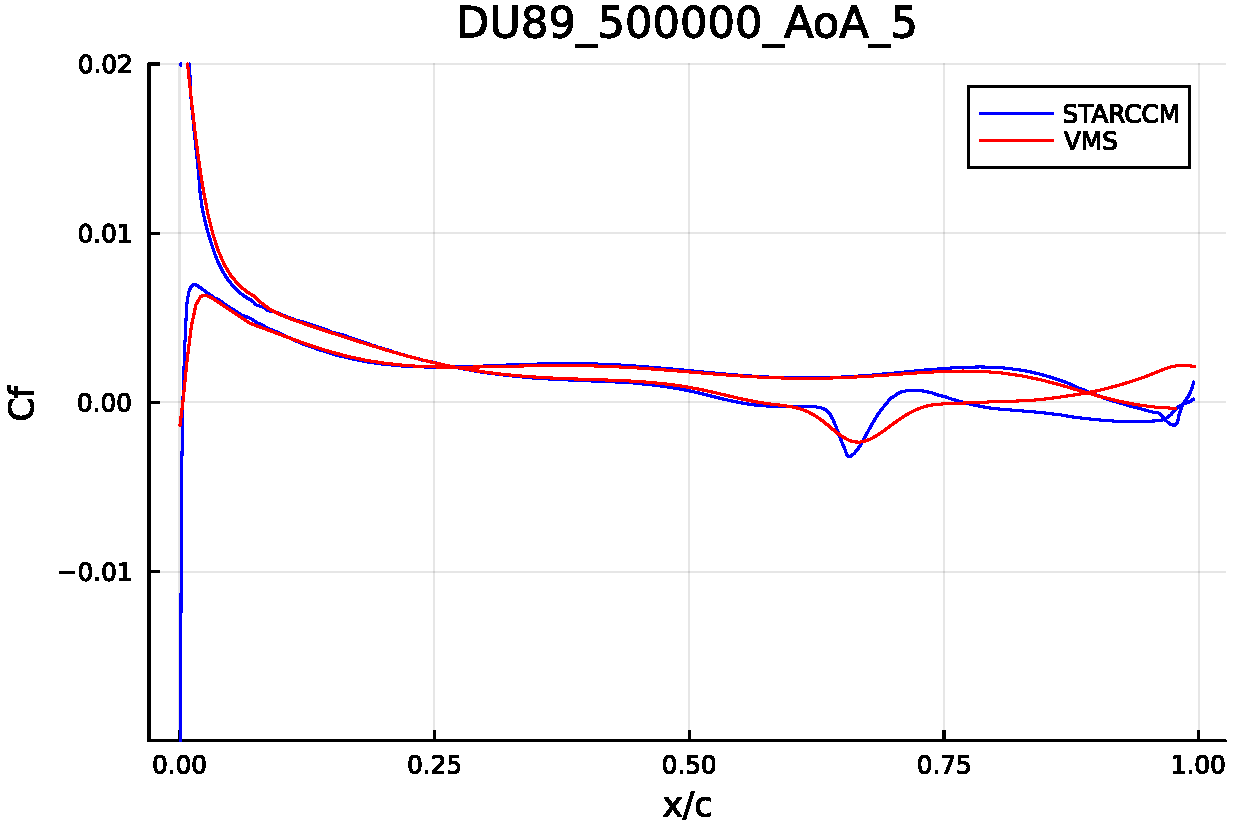
\includegraphics[width=\textwidth]{DU89_500000_AoA_5_Cf.pdf}
    \end{subfigure}
          \hfill
     \begin{subfigure}[h]{0.45\textwidth}
      \centering
         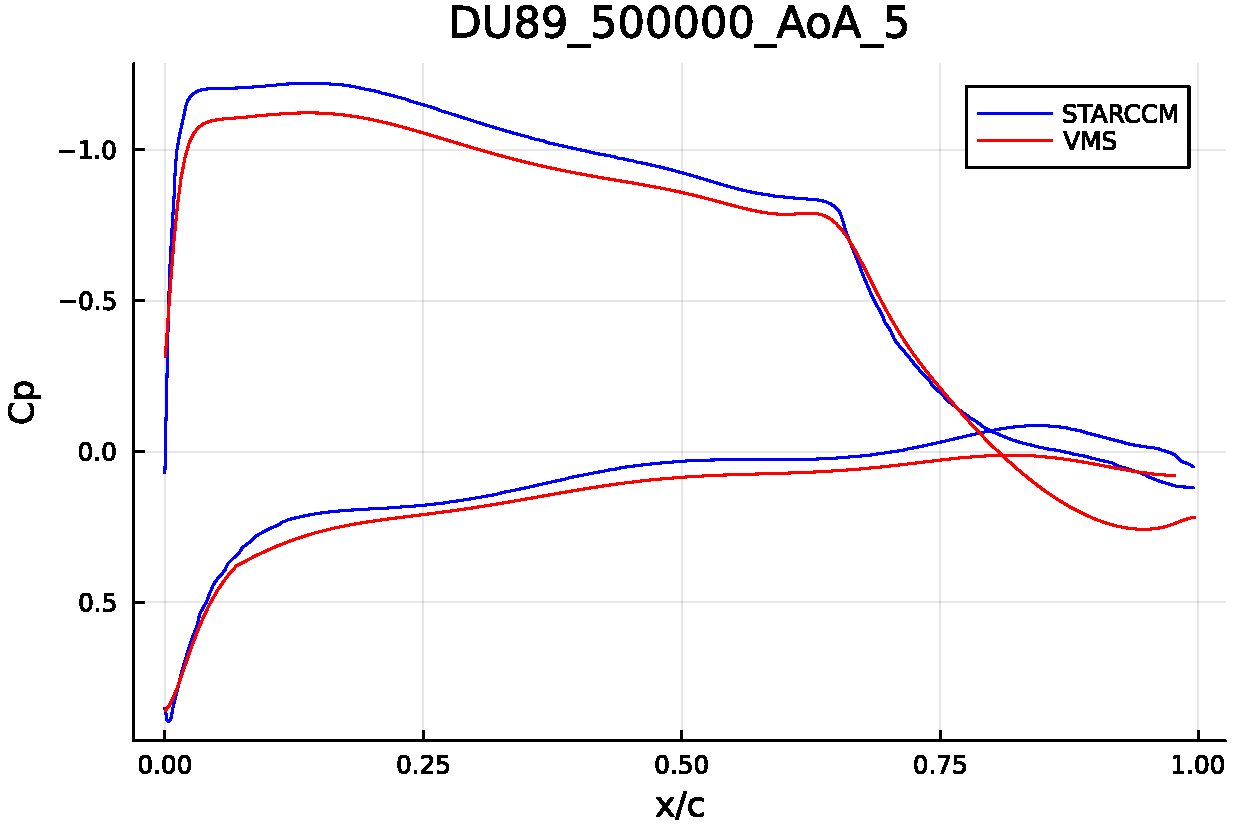
\includegraphics[width=\textwidth]{DU89_500000_AoA_5_Cp.pdf}
     \end{subfigure}
     \end{figure} 
 \end{frame}

